%===========================================================
%                              Choix de thématique
%===========================================================
% Une des quatre options 'parallelisme', 'architecture', 'systeme' 
% 'tempsreel' doit être utilisée avec le style compas2021
\documentclass[sigconf,review]{acmart}

\usepackage{listings}
\usepackage{algorithmicx}
\usepackage[noend]{algpseudocode}
\usepackage{algorithm,hhline}
\usepackage{graphicx}
\usepackage{wrapfig}
\usepackage{subcaption}
\usepackage{color}

\definecolor{light-gray}{gray}{0.80}
%===========================================================
%                               Title
%===========================================================
\definecolor{dkgreen}{rgb}{0,0.6,0}
\definecolor{gray}{rgb}{0.5,0.5,0.5}
\definecolor{mauve}{rgb}{0.58,0,0.82}

\lstset{frame=tb,
  language=C,
  aboveskip=3mm,
  belowskip=3mm,
  showstringspaces=false,
  columns=flexible,
  basicstyle={\small\ttfamily},
  numbers=none,
  numberstyle=\tiny\color{gray},
  keywordstyle=\color{blue},
  commentstyle=\color{dkgreen},
  stringstyle=\color{mauve},
  breaklines=true,
  breakatwhitespace=true,
  tabsize=3
}
\lstset{emph={%  
    in%
    },emphstyle={\color{red}\bfseries}%
}%
\begin{document}
\bibliographystyle{plain}

\lstset{
  language=C,
  basicstyle=\tiny\ttfamily,
%  numbers=left,
%  xleftmargin=2em,
  frame=single,
%  framexleftmargin=2em,
  escapeinside={(*}{*)}
}

\title{Exploring Vectorization and unrolling with SMT}

\author{Denis Barthou}
\affiliation{\institution{Bordeaux Institute of Technology} \city{Bordeaux} \country{France}}
\author{Edgar Baucher}
\affiliation{\institution{Bordeaux Institute of Technology} \city{Bordeaux} \country{France}}
\author{Ahmed-Manaf Dhamani}
\affiliation{\institution{Bordeaux Institute of Technology} \city{Bordeaux} \country{France}}
\author{William Jalby}
\affiliation{\institution{University of Versailles Saint Quentin} \city{Versailles} \country{France}}


%\date{\today}

%===========================================================         %
%Abstract
%===========================================================  
\begin{abstract}
  
\end{abstract}
\keywords{}

\maketitle



\section{Introduction}
The high performance kernels require multiple optimizations. We do not
focus particularly on codes from libraries, but rather on kernels from
applications. One of the objectives is to study how to generate
efficient source code, while still keeping the code portable,
understandable by users and allowing composition. As a counterpart, we
may not wish to reach top performance but this would be suficient to
stay close to it (let us say 80\% of the top performance) if this
allows portability, maintenance and composability.

Many optimizations at the loop level and targeting cache/memory
hierarchy are well known and can be handled by dedicated compiler
optimizations. We will focus here on code optimizations for codes that
run in a tile of data fitting in cache (or that does not have
reuse). Essentially, the optimizations concerned are instruction
scheduling (notably through loop transformations), SIMDization,
register allocation. Besides, we assume the user selects SIMD
instructions, using for instance a library such as the C++ MIPP
wrapper \cite{mipp}. We therefore focus on a very narrow optimization
space, playing only with loop unrolling and letting to the compiler
deal with instruction scheduling and register allocation.  The
advantage of this approach is that this is only source code and
compiler variations, hence allows composition of codes.  The
particularities of the kernels and vectorization with MIPP are
recalled here:
\begin{itemize}
  \item Vector instructions will be parametrized by their length VL (expressed in elements) so the code should be generic and cover all possible Vector Lengths
\item All instructions will be not differentiated with respect to DP versus SP. It will be the optimizer which will take care of that specialization.
\item All arithmetic instructions will operate between registers (à la ARM): no operand coming from memory can be used in an arithmetic instruction. Potentially, this characteristic increases register pressure where a combined load/arithmetic operation could avoid unnecessary use of registers. This characteristic is compatible though with C++ library such as MIPP. 
\item All arithmetic instructions will use only Vector Registers as main operands no scalar registers can be used. This will require the use of Broadcast instructions to promote a scalar to vector.
\item We will use a Vector Reduction (denoted VRED) instruction capable of summing all of the components of a vector register. Such an instruction is available in ARM ISA but currently it requires a chain of between 4 and 6 instructions on X86
\item The code to by duplicated (through unrolling) will be enclosed between curly brackets. 
\item The instruction selection for vectorized code is assumed to be done by the user through MIPP. Indeed, while efficient instruction selection methods exist in current compilers, this is still limited to linear algebra codes. MIPP (or existing alternatives) removes this issue by proposing a wider access to intrinsics SIMD instructions.
\end{itemize}
Instruction scheduling and register allocation are two key optimizations that must be performed in order to reach high level performance code. Two possibilities: either the user specifies in high level ASM both of them, or the compiler is in charge. 

\section{Matrix product, stored row-wise}
The matrx code is a kernel for libraries, but still there may be occurences of special matrix sizes that are not perfectly addressed by libraries. We will start with small rectangular bloc sizes first. In the code presented in Fig.\ref{fig:gemm}, all loops are potentially unrolled. Variables \texttt{ui}, \texttt{uj}, \texttt{uk}
are indices corresponding to the unrolling factors. The unrolling on k
produces a sequence of FMAs. This does not improve ILP for FMA but
this enhances register reuse and can help to hide other instruction
latencies (loads).  There is no tail code on purpose, the sizes BI,
BJ, BK are adjusted to the unrolling factors, while still keeping the
global size of matrices A,B and C within 5\% of the chosen global
size, for all unrolling factors.  The unrolling factors from 1 to 15
have been explored to evaluate the capacity of the compilers to
allocate registers and reschedule. We have limited the exploration of
the register block size $UI*UJ+UI*UK+UJ*UK$ so that it does not exceed
twice the amount of SIMD registers (so 64 for AVX512, 32 for AVX), and
$UJ*VL$ should not exceed the size of the dimension BJ.  The type of the elements are defined by \texttt{TYPE} . The above code
is written using a template mechanism that is instantiated
into C++ code for all unrolling factors.  The first machine of the
evaluation is an Intel Cascade Lake 6230R with AVX-512. The compilers
evaluated are, with flag -O3: icc version 19.1.3.304,  Clang 15 with 3 register allocation methods, greedy
(base), basic and PBQP, and GCC version 11.9. icc version 2021
(dpc++ OneAPI) is based on Clang 15 and does not exhibit differences with Clang 15 greedy. 


\begin{figure}
  \begin{lstlisting}
for (int i=0;i<BLOCKI;i+=ui) {                
  for (int j=0;j<BLOCKJ;j+= uj*nv) {           
    { ii in [0,ui],jj in [0,uj]:
        mipp::Reg<TYPE> c_ii,jj;
        c_{ii,jj}.load(&C[(i + ii )*BLOCKJ + j + jj *nv]);
    }                
    for (int k=0;k<BLOCKK;k+= uk ) {            
      { ii in [0,ui],kk in [0,uk]:
          mipp::Reg<TYPE> a{{ ii }}{{ kk }};
          a_{ii,kk} = mipp::set1<TYPE>(A[(i + ii )*BLOCKK+k+ kk ]);
      }
      { jj in [0,uj],kk in [0,uk]:
          mipp::Reg<TYPE> b{{ kk }}{{ jj }};
          b_{kk,jj}.load(&B[(k+ kk )*BLOCKJ + j + jj*nv]);
      }    
      { ii in [0,ui], jj in [0,uj] :
          c_{ii,jj} = { k in [0,uk]: mipp::fmadd(a_ii,kk, b_kk,jj, } , c_ii,jj  { k in [0,uk]: ) };
      }
    }
    { ii in [0,ui],jj in [0,uj]:
        c_ii,jj.store(&C[(i+ ii )*BLOCKJ + j + ( jj )*nv]);      
    }
  }
}
  \end{lstlisting}
  \caption{Matrix product vectorized and unrolled\label{fig:gemm}. \texttt{in} constructs correspond to unrolled statements/expressions. }
\end{figure}


\subsection{Performance evaluation with double on Intel CascadeLake}
\begin{figure*}[ht]
%  \begin{subfigure}[h]{0.45\textwidth}
%  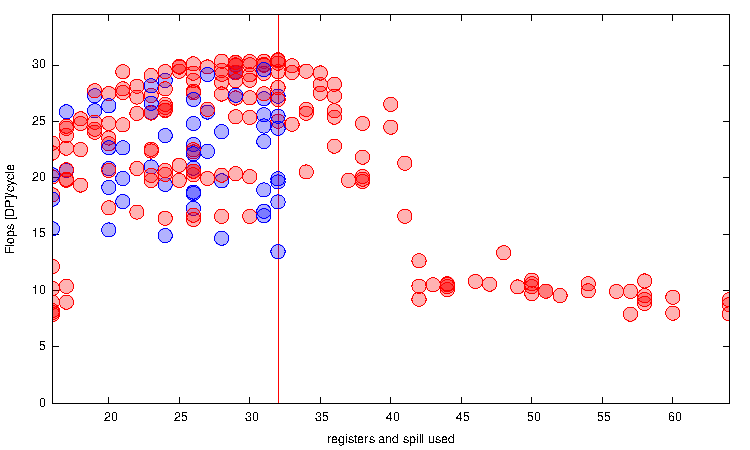
\includegraphics[width=\textwidth]{../benches/gemm/cascadelake-64x256x64/icc-2021.2.0.pdf}
%  \caption{icc 2021.2.0}
%  \end{subfigure}
  \begin{subfigure}[h]{0.45\textwidth}  
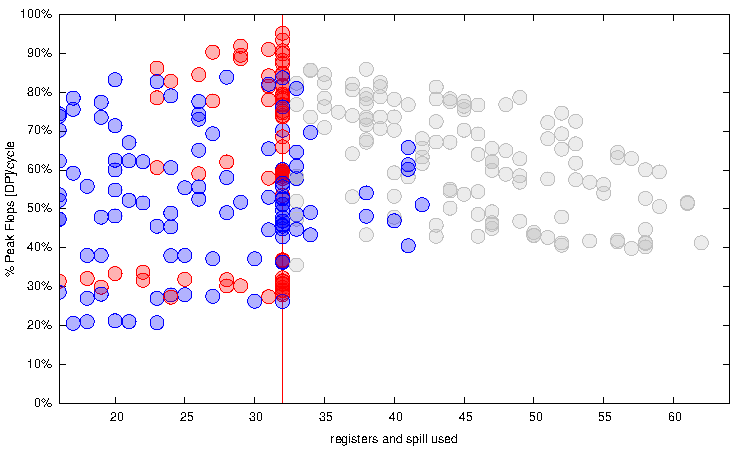
\includegraphics[width=\textwidth]{../benches/gemm/cascadelake-64x256x64/icc-19.1.3.pdf}
  \caption{icc 19.1.3}
  \end{subfigure}
  \begin{subfigure}[h]{0.45\textwidth}  
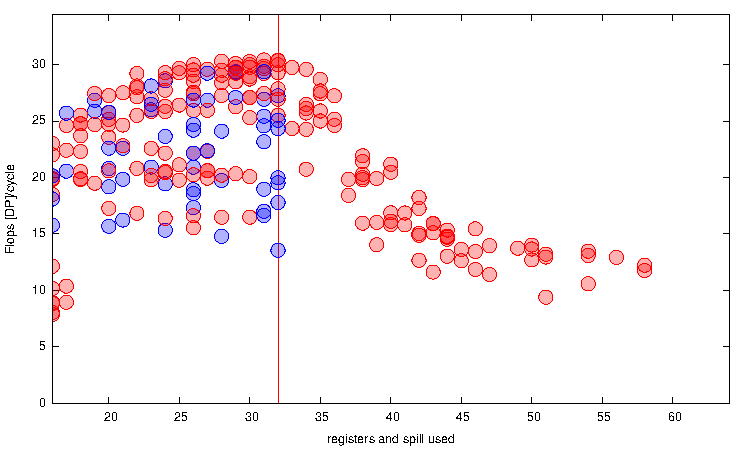
\includegraphics[width=\textwidth]{../benches/gemm/cascadelake-64x256x64/pbqp.pdf}
  \caption{Clang 15 with PBQP register allocation}
  \end{subfigure}
  \begin{subfigure}[h]{0.45\textwidth}  
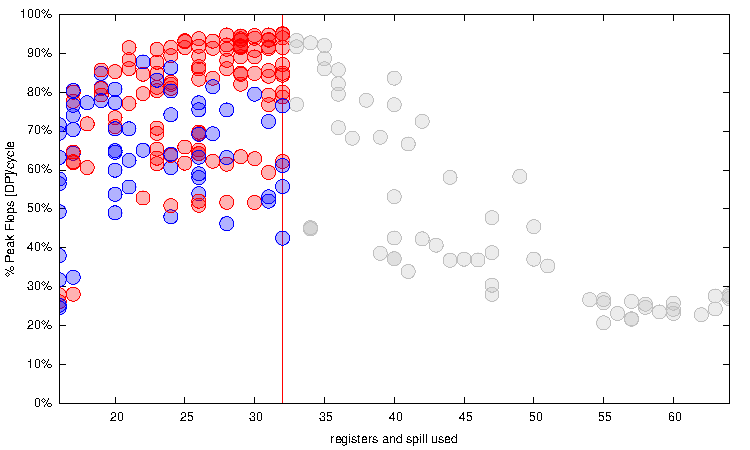
\includegraphics[width=\textwidth]{../benches/gemm/cascadelake-64x256x64/greedy.pdf}
  \caption{Clang 15 with greedy register allocation}
  \end{subfigure}
  \begin{subfigure}[h]{0.45\textwidth}  
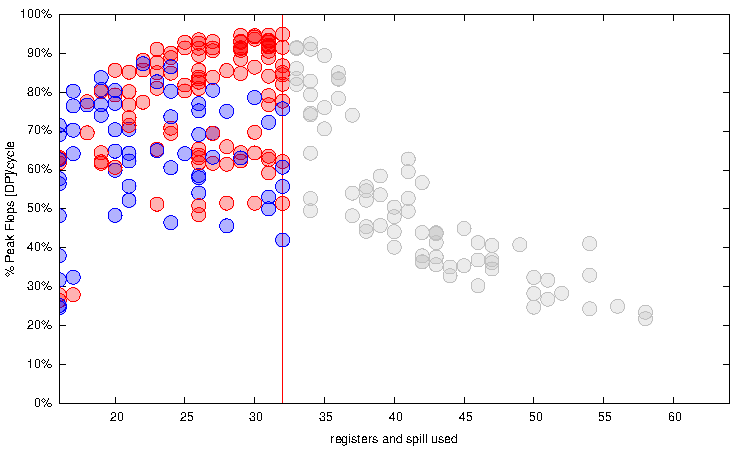
\includegraphics[width=\textwidth]{../benches/gemm/cascadelake-64x256x64/basic.pdf}
  \caption{Clang 15 with basic register allocation}
  \end{subfigure}
  \begin{subfigure}[h]{0.45\textwidth}  
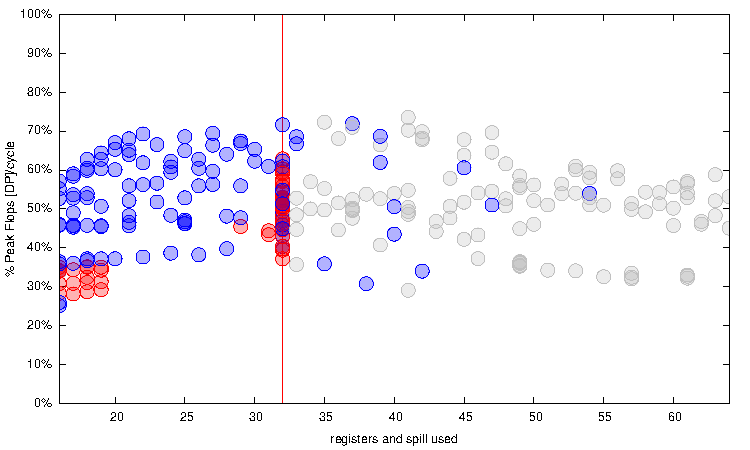
\includegraphics[width=\textwidth]{../benches/gemm/cascadelake-64x256x64/gcc-11.9.pdf}
  \caption{GCC 11.9}
  \end{subfigure}\hfill ~
  \caption{Block DGEMM Performance used on Intel CascadeLake with different compilers. Performance is given in \% of peak flops/cycle (here 32). The block (BI,BK,BJ) is 64x256x64. Each code represent a different register block size, obtained through the three unrolling factors. Codes with register block size $\leq 32$ are in blue (fit in register whatever the schedule), others in red.  \label{fig:cascadelake}}
\end{figure*}
 For all plots in Fig.\ref{fig:cascadelake}, the same codes with the same vectorization expressed with MIPP are
compiled. All codes are tested 40 times, the best performance is shown. Only one memory allocation is used for all tests. Points shown in blue correspond to codes that should not require
more SIMD registers than the physical registers (32 here, shown by the vertical red line), whatever
the scheduling chosen by the compiler. This is not the case for codes
shown in red, some schedules may manage to use only registers while
others will require spill code. The graphs show performance w.r.t. the
cumulated register count and spill used by the code. For instance, a value of 40 registers and
spill used indicates that the compiler was able to use all 32
registers and 8 additional spaces on the stack for spill. With the exception of
GCC, other compilers manage to allocate less than 32 registers for all
blue codes. The max performance on this machine is normally 32 flops/cycles (with 2 FMAs operating on AVX512 vectors).  

There is no significant difference between icc version 2021 and Clang
15, either greedy or PBQP register allocations. This is expected since
icc now is based on LLVM. GCC however fails significanlty, reaching
only 24 flop/cycle while other compilers reach 30-31 flop/cycle.  For
the following experiments, only Clang 15 with greedy register
allocation is considered.

We observe that the best performance is reached with Clang 15 and
icc-19.1.3 when the codes use exactly 32 registers. With gcc-11.9, the
best code suing exactly 32 registers is among the best codes obtained
with this compiler.  Tables shown in Figure \ref{fig:tables} show the
performance of all codes using exactly 32 registers, no spill. The
block size refers to the size taken by the input matrices manipulated
in the inner loop, in number of vectors. Sizes larger than 32 imply that the compiler has introduced some additional loads during the computation and reuses SIMD registers. We observe that the best codes are different from one compiler to the other. 

\begin{figure*}[ht]
% For clang 15
{    \scriptsize
    \begin{tabular}{|c|c|c|}
      \hline
      \multicolumn{3}{|c|}{Code performance with Clang} \\
      \hline
      Unrolling (ixkxj) & flop/cycle & block size \\
      \hline
      2x7x2 & 13.61  & 32\\
2x4x4 & 17.85  & 32\\
2x2x7 & 19.92  & 32\\
4x4x2 & 19.58  & 32\\
7x2x2 & 24.50  & 32\\
3x3x6 & 25.62  & 45\\
4x2x4 & 25.23  & 32\\
10x1x2 & 27.19  & 32\\
7x4x2 & 27.03  & 50\\
8x4x2 & 27.90  & 56\\
10x2x2 & 29.29  & 44\\
6x4x3 & 30.10  & 54\\
7x3x3 & 30.42  & 51\\
8x2x3 & 30.44  & 46\\
\hline
\end{tabular}
% For icc
    \begin{tabular}{|c|c|c|c|}
      \hline
      \multicolumn{3}{|c|}{Code performance with icc 19.1.3} \\
      \hline
      Unrolling (ixkxj) & flop/cycle  & block size \\
      \hline
3x2x6 & 25.34  & 36\\
3x2x7 & 25.16  & 41\\
3x2x8 & 25.47  & 46\\
3x1x8 & 26.21  & 35\\
4x3x4 & 26.10  & 40\\
7x2x2 & 26.81 & 32 \\
4x2x4 & 27.18  & 32\\
5x2x4 & 27.97  & 38\\
6x2x3 & 27.11  & 36\\
4x1x6 & 28.78  & 34\\
4x2x5 & 28.23  & 38\\
10x1x2 & 29.02  & 32\\
5x1x5 & 29.91  & 35\\
6x1x4 & 30.47  & 34\\
\hline
    \end{tabular}
% For icc
    \begin{tabular}{|c|c|c|c|}
      \hline
      \multicolumn{3}{|c|}{Code performance with gcc 11.9} \\
      \hline
      Unrolling (ixkxj) & flop/cycle  & block size \\
      \hline
2x5x3 & 17.42  & 31\\
2x5x4 & 17.31  & 38\\
3x6x2 & 17.55  & 36\\
2x2x6 & 18.41  & 28\\
3x3x5 & 18.36  & 39\\
3x5x3 & 18.93  & 39\\
3x5x4 & 18.27  & 47\\
2x4x4 & 19.30  & 32\\
3x2x5 & 19.07  & 31\\
3x4x3 & 19.96  & 33\\
3x4x4 & 19.31  & 40\\
3x5x2 & 19.49  & 31\\
3x3x4 & 20.13  & 33\\
5x3x2 & 22.94  & 31\\
\hline
    \end{tabular}
}
\caption{Performance of the best 14 codes with Clang15,  icc 19.1.3 and gcc 11.9. Only codes using 32 registers and 0 spill are considered here\label{fig:tables}}
\end{figure*}

Figure \ref{fig:cascadelakecorrelation}  shows the correlation between the codes compiled by the three compilers. One dot corresponds to the same source code, with the same unrolling factors. This confirms that the correlation is rather weak. 

\begin{figure*}[ht]
  \begin{subfigure}[h]{0.45\textwidth}
  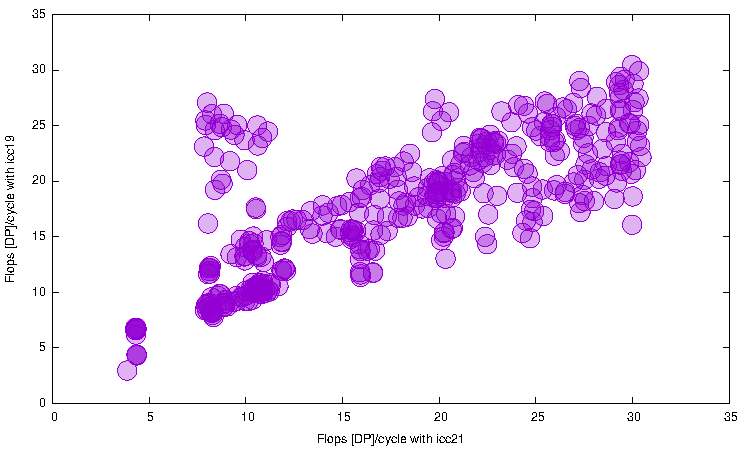
\includegraphics[width=\textwidth]{../benches/gemm/cascadelake-64x256x64/icc21xicc19.pdf}
  \caption{Clang 15 compared to icc 19.1.3}
  \end{subfigure}
  \begin{subfigure}[h]{0.45\textwidth}  
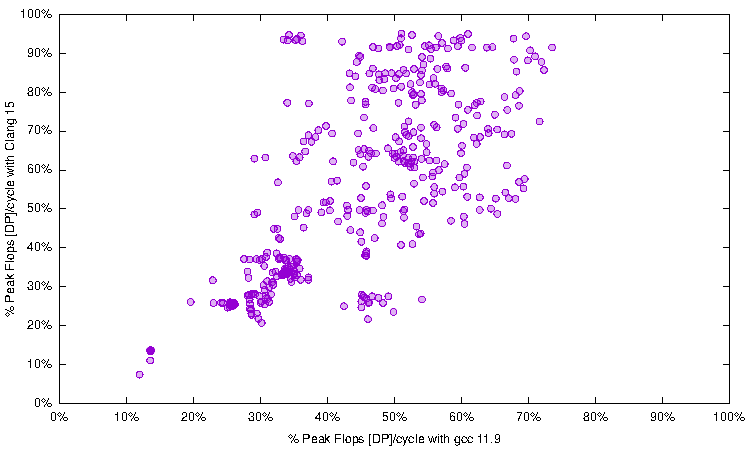
\includegraphics[width=\textwidth]{../benches/gemm/cascadelake-64x256x64/gccxgreedy.pdf}
  \caption{Clang 15 compared to gcc 11.9}
  \end{subfigure}
  \caption{Correlation of code performance on CascadeLake between different compilers.\label{fig:cascadelakecorrelation}}
\end{figure*}

Finally, Figure \ref{fig:cascadelakeloc} shows for a given number of
source code lines, the performance obtained. Surprisingly, performance
culminates with 90 loc and then it degrades when the number of source
code lines. Note that the unrolling factor on k, creating a long
sequence of FMAs, is assumed to be on one single line of code.
\begin{figure*}[ht]
  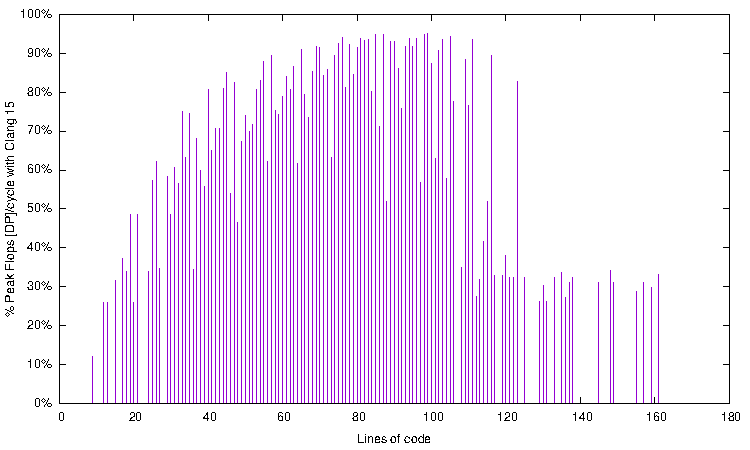
\includegraphics[width=0.45\textwidth]{../benches/gemm/cascadelake-64x256x64/icc21loc.pdf}
  \caption{Performance wrt lines of source code\label{fig:cascadelakeloc}}
\end{figure*}


\subsection{Performance evaluation with double on ArmThunderX2}
The codes considered are exactly the same as before (portability).  Due to the architecture of the processor, supporting a SMT of 4, we compared performance for a single thread and performance with 4 threads, both on a single core. 

\begin{figure*}[ht]
  \begin{subfigure}[h]{0.45\textwidth}
  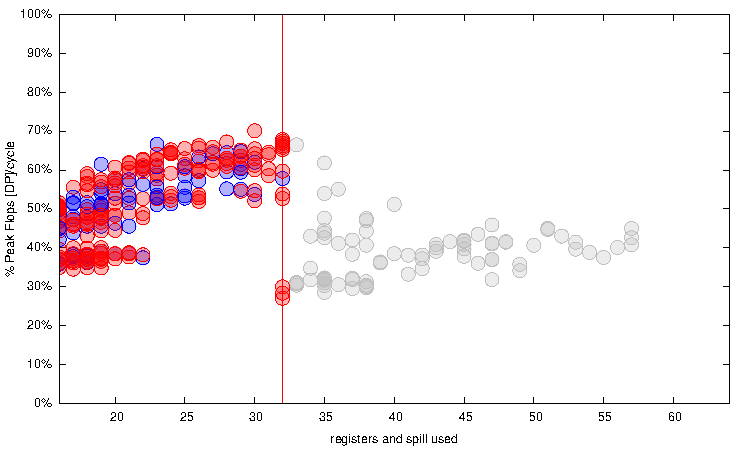
\includegraphics[width=\textwidth]{../benches/gemm/arm-64x256x64/greedy.pdf}
  \caption{clang 15}
  \end{subfigure}
  \begin{subfigure}[h]{0.45\textwidth}  
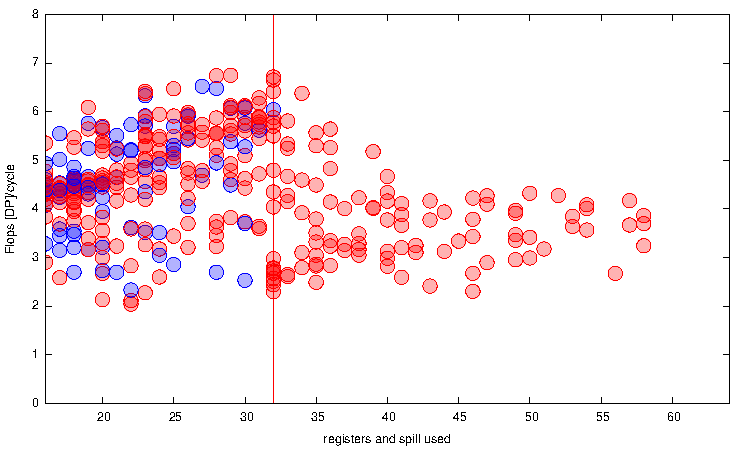
\includegraphics[width=\textwidth]{../benches/gemm/arm-64x256x64/openmp.pdf}
  \caption{clang 15 with OpenMP, SMT of 4}
  \end{subfigure}
  \begin{subfigure}[h]{0.45\textwidth}  
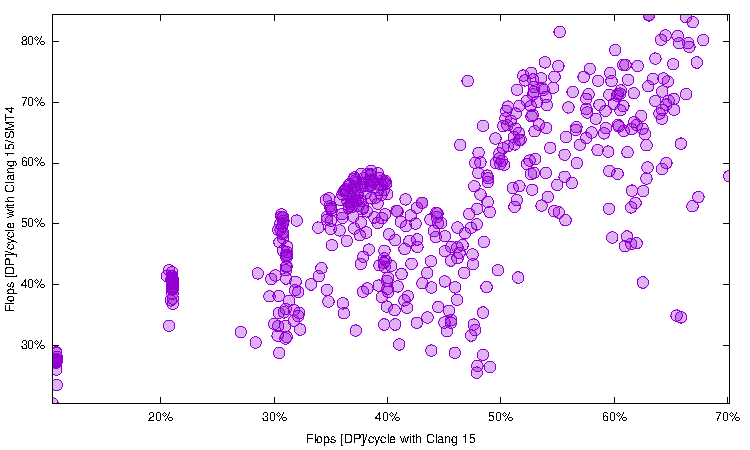
\includegraphics[width=\textwidth]{../benches/gemm/arm-64x256x64/clangxsmt.pdf}
  \caption{Correlation between Clang 15 without and with SMT4}
  \end{subfigure}
  \caption{Block DGEMM Performance used on Arm ThunderX2 with different compilers. Performance is given in \% of peak flops/cycle (here 8). The block (BI,BK,BJ) is 64x256x64. Each code represent a different register block size, obtained through the three unrolling factors. Codes with register block size $\leq 32$ are in blue (fit in register whatever the schedule), others in red. (c) show correlation between the two plots. \label{fig:cascadelake}}
\end{figure*}

\section{Related Works}
\section{Conclusion}
\label{sec:conclusion}

\bibliography{biblio}

\end{document}
